\chapter{Other Approaches}
\label{chap:otherapproaches}
In this chapter, we describe both the Linux reference implementation of LUKS2 and the two disk encryption technologies that are featured in the performance comparison in \autoref{chap:performance}.

\section{Linux Kernel Implementation of LUKS2}
\label{chap:otherapproaches.linux}
To compare the architecture of our driver (see \autoref{chap:ourapproach.final}) to that of the Linux reference implementation, the latter will be described in this section. To see how the user space part of this implementation works, we will take a look at the source code of the \texttt{cryptsetup} tool. The work of looking through the Linux kernel source code and creating a high-level overview has already been done in \cite{Korchagin2020}.

\subsection{The Linux Kernel Device Mapper}
\label{chap:otherapproaches.linux.dm}
The reference implementation uses the Linux kernel's device mapper \cite{Dmcrypt2020}. This is a kernel driver that allows creating virtual devices in layers. One such layer is known as a \emph{target}. A layer can be thought of as the Linux equivalent of a Windows file system filter driver.\footnote{\label{fn:otherapproaches.linux.dmtargetdriver} This comparison holds as far as that the functionality of target is implemented by a kernel driver. It is also possible to implement new targets, as done e.g. in \cite{Barker2019}.} The device mapper comes with many different available targets, including \cite{Linux}:
\begin{descitemize}
	\item[\texttt{zero}] This target always returns zeroes for all reads and silently discards all writes. It is similar to Linux' \texttt{/dev/zero}, but in contrast to that this is a block device, not a character device.\footnote{\label{fn:otherapproaches.linux.charvsblock} The difference is that character devices read and write a stream of individual byes, and block devices read and write blocks (usually 512 bytes) \cite{Corbet2005}.}
	\item[\texttt{linear}] This target maps a range of blocks of the virtual device to an existing device. Described in more detail: map the block range $N$ to $N+L$ of the virtual device to the block range $M$ to $M+L$ of device $X$.
	\item[\texttt{snapshot}] This target creates a copy-on-write snapshot of a device. These snapshots are ``mountable, saved states of the block device which are also writable without interfering with the original content.'' \cite{Linux}
	\item[\texttt{crypt}] This target performs transparent encryption of a device (writes are encrypted, reads are decrypted). This is what the LUKS2 reference implementation uses. The encryption is done via the Linux kernel's crypto API, which offers a variety of different encryption schemes. This interface is described in more detail in \cite{Linux}.
\end{descitemize}

The configuration of a virtual device happens via a \emph{mapping table}. The general format is described in \autoref{fig:otherapproaches.linux.mappingtable}, and \autoref{fig:otherapproaches.linux.dmcryptparameters} describes the parameter format for the \texttt{crypt} target.

Outside of the mapping table, the device mapper's targets are usually written with the \texttt{dm-} prefix, e.g. we write \texttt{dm-crypt} for the \texttt{crypt} target.

\begin{figure}[htb!]
	\center
	\begin{mdframed}
		\texttt{<start block> <size> <target name> <target parameters>}
	\end{mdframed}
	\caption[
		Linux device mapper mapping table entry format
	]{
		Linux device mapper mapping table entry format (modified after \cite{Dmcrypt2020}). The \texttt{start block} is the first block of the virtual device that this mapping applies to. \texttt{size} indicates the number of blocks, including the start block, that this mapping is for. \texttt{target name} specifies the device mapper target that will be used. The \texttt{target parameters} are specific to each of the different targets. The \texttt{crypt} target's parameters are described in \autoref{fig:otherapproaches.linux.dmcryptparameters}.\\
		The full mapping for a virtual device can contain multiple entries, each in its own line. It is possible to combine different targets. The following example shows a 1024 block virtual device, whose first half is mapped using the \texttt{linear} target, and whose second half is mapped using the \texttt{crypt} target:\\
		\texttt{0\space\space\space{}512 linear <linear parameters>}\\
		\texttt{512 512 crypt\space\space{}<crypt parameters>}
	}
	\label{fig:otherapproaches.linux.mappingtable}
\end{figure}

\begin{figure}[htb!]
	\center
	\begin{mdframed}
		\texttt{<cipher> <key> <iv offset> <device path> <offset> [<\#opt> <opt> <...>]}
	\end{mdframed}
	\caption[
		\texttt{dm-crypt} target parameter format
	]{
		\texttt{dm-crypt} target parameter format (modified after \cite{Dmcrypt2020}). \texttt{cipher} specifies the encryption cipher that is used, in the following format: \texttt{cipher-chainmode-ivmode[:ivopts]}. See \autoref{chap:background.luks2.using} for more on ciphers, chain modes (also known as block cipher modes), and IVs. \autoref{tbl:background.luks2.encryptionalgorithms} also lists examples of available encryption algorithms. \texttt{key} is the key used for the specified cipher. It can either be in hexadecimal notation, or a reference to a key in the kernel keyring (more on this shortly). The \texttt{iv offset} is a constant offset that is added to the sector number to create the IV. The \texttt{device path} determines the device the encrypted data is stored on, either by giving its path (e.g. \texttt{/dev/sda1}) or its major and minor number (e.g. \texttt{8:16}, see \cite{Corbet2005} for more on these). The \texttt{offset} gives the first sector on the specified device containing the encrypted data. Additionally, optional parameters can be specified after these required parameters, e.g. the disk's sector size, preceded by the count of optional parameters.
	}
	\label{fig:otherapproaches.linux.dmcryptparameters}
\end{figure}

\autoref{fig:otherapproaches.linux.dmcryptparameters} mentioned the \emph{kernel keyring} (also known as the kernel key retention service). It is provided by the Linux kernel to cache keys and other secrets for usage by other kernel components. Keys have different attributes, including a key type, a name (also called a description), and a unique serial number. Depending on the key type and a user's permissions, keys can also be accessed from user space using that serial. The serial can be obtained by searching for a key using its type and name. Kernel services can register new key types, supplementary to some already defined types. These include \cite{Linux}\cite{ManKeyrings}:
\begin{descitemize}
	\item[\texttt{keyring}] A key of this type contains a list of links to other keys, including other keyrings.
	\item[\texttt{user}] A key of this type contains a payload of arbitrary binary data (up to 32767 bytes) and can be accessed and modified from user space. Because of this, keys of this type are not intended to be used by the kernel.
	\item[\texttt{logon}] This is similar to the \texttt{user} type, but keys of this type can only be read by the kernel. It is however possible to create or update them from user space. A \texttt{logon} key's description must start with a prefix followed by a colon, with the prefix denoting which service the key belongs to.
\end{descitemize}

The format of the \texttt{key} parameter from \autoref{fig:otherapproaches.linux.dmcryptparameters} when using the kernel keyring is: \texttt{:<size>:<type>:<description>}. \texttt{size} is the key size in bytes, and \texttt{type} and \texttt{description} are the key's type and description, respectively \cite{Dmcrypt2020}. See \autoref{chap:otherapproaches.linux.cryptsetup} for an example value of this parameter, created by the \texttt{cryptsetup} tool.

As already mentioned, \texttt{dm-crypt} uses the Linux kernel's crypto API for the de- and encryption of reads and writes. \autoref{fig:otherapproaches.linux.dmcryptio} shows the flow of I/O operations through different parts of \texttt{dm-crypt} and the crypto API. \cite{Korchagin2020} experimented with skipping some of the queues shown in the figure, and found significantly increased throughput for some hardware configurations and use cases. They therefore implemented the possibility to configure \texttt{dm-crypt} to queue less operations. This is done via optional parameters (see \autoref{fig:otherapproaches.linux.dmcryptparameters}), and can be used since Linux 5.9 \cite{Dmcrypt2020}.

\begin{figure}[htb!]
	\center
	\small
	\begin{tikzpicture}[
		read/.style={
			arrow,
			very thick,
			draw=tBlue,
		},
		write/.style={
			arrow,
			very thick,
			draw=tPink,
		},
	]
		\node[rect, dashed, rounded corners=10pt, from={0, 1.5 to 6.5,  7}] {};
		\node[rect, dashed, rounded corners=10pt, from={8, 1.5 to 14.5, 7}] {};

		\foreach \x\y in {2.25/6,2.25/2,4/4,10.4/5.4,10.2/5.2,10/5} {
			\node[rect, draw=gray!70, fill=gray!30, minimum width=0.5cm, minimum height=0.5cm] at (\x,     \y) {};
			\node[rect, draw=gray!70, fill=gray!30, minimum width=0.5cm, minimum height=0.5cm] at (\x+0.5, \y) {};
			\node[rect, draw=gray!70, fill=gray!30, minimum width=0.5cm, minimum height=0.5cm] at (\x+1.0, \y) {};
			\node[rect, draw=gray!70, fill=gray!30, minimum width=0.5cm, minimum height=0.5cm] at (\x+1.5, \y) {};
		}

		\node[rect, draw=gray!70, fill=gray!30, from={1,    4   to 1.5,  4.5}] {};
		\node[rect, draw=gray!70, fill=red,     from={0.75, 3.5 to 1.25, 4}]   {};
		\node[rect, draw=gray!70, fill=black,   from={1.25, 3.5 to 1.75, 4}]   {};

		\node at (1.25,  4.75) {write\_tree};
		\node at (3,     2.5)  {dmcrypt\_write};
		\node at (3,     6.5)  {kcryptd\_io};
		\node at (4.7,   4.5)  {kcryptd};
		\node at (11.15, 5.9)  {cryptd};

		\node[anchor=north west, xshift=2pt, yshift=-2pt] at (0, 7) {\footnotesize\textit{dm-crypt}};
		\node[anchor=north west, xshift=2pt, yshift=-2pt] at (8, 7) {\footnotesize\textit{Crypto API}};

		\node[rect, fill=tOrng, rounded corners=4pt, from={4.75, 7.5 to 9.75, 8.5}] (fs)  {File system driver};
		\node[rect, fill=tPurp, rounded corners=4pt, from={4.75, 0   to 9.75, 1}]   (dev) {Device driver};

		\draw[read] (fs.west)    -| (4.375, 6)    -- (4, 6);
		\draw[read] (3, 5.75)    -- (3, 3)        -| (5.25, 1);
		\draw[read] (dev.east)   -| (10.25, 3.25) -| (4.75, 3.75);
		\draw[read] (5.5, 3.75)  -- (5.5, 3.5)    -| (11.5, 4.75);
		\draw[read] (11.9, 5.65) |- (fs.east);
		\node[anchor=east] at (4.375, 8) {\textcolor{tBlue!90!black}{read}};

		\draw[write] (fs.south)   |- (5.5, 5.875) -- (5.5, 4.25);
		\draw[write] (5.75, 4)    -| (10.5, 4.75);
		\draw[write] (9.75, 5)    -- (3.25, 5)    |- (1.5, 4.25);
		\draw[write] (1.25, 3.5)  |- (2, 2);
		\draw[write] (3.75, 1.75) |- (dev.west);
		\node[anchor=north west] at (fs.south) {\textcolor{tPink!90!black}{write}};
	\end{tikzpicture}
	\caption[
		\texttt{dm-crypt} and Linux kernel crypto IO traverse path
	]{
		\texttt{dm-crypt} and Linux kernel crypto IO traverse path (modified after \cite{Korchagin2020}). A write request from the file system driver first moves into the \texttt{kcryptd} workqueue. This queue takes care of doing the encryption at some later, more convenient point in time (see \cite{Linux} for more details). The Linux kernel crypto API does the actual encryption work, and it also may use internal queues. The encrypted write requests are then sorted by \texttt{dm-crypt} using a red-black tree and are sent to the device driver via another workqueue. \\
		For read requests, the encrypted data is retrieved from the device driver using the \texttt{kcryptd\_io} workqueue. When this data arrives, it is scheduled for decryption in the already mentioned \texttt{kcryptd} queue. When the kernel crypto API has done its work, the decrypted data is ready for the file system driver.
	}
	\label{fig:otherapproaches.linux.dmcryptio}
\end{figure}

\subsection{The \texttt{cryptsetup} Command Line Utility}
\label{chap:otherapproaches.linux.cryptsetup}
Manually configuring the device mapper to work with encrypted partitions is impractical. Therefore, \texttt{dm-crypt} is accompanied by the \texttt{cryptsetup} command line utility. Its purpose is, given an encrypted volume, to automatically generate the appropriate \texttt{dm-crypt} configuration and send it to the kernel. It supports multiple different encryption technologies, including \cite{ManCryptsetup}:
\begin{itemize}
	\item LUKS and LUKS2 (see \autoref{chap:background.luks2});
	\item TrueCrypt and VeraCrypt (see \autoref{chap:otherapproaches.veracrypt});
	\item BitLocker (see \autoref{chap:otherapproaches.bitlocker}). The support for it is relatively new and still in experimental status.
\end{itemize}

For LUKS and LUKS2, there is additional functionality available, including formatting new partitions, upgrading a LUKS partition to LUKS2, and adding new keyslots (which have been described in \autoref{chap:background.luks2}) \cite{ManCryptsetup}.

To illustrate the usual workflow and explain some details ``hands-on'', we will use the following example: suppose we want to use the LUKS2-encrypted partition located at \texttt{/dev/sda1}. We will describe how to make the decrypted partition available, how to mount the contained file system, and how to unmount it and relock the partition again. For the first step, we will also take a look at parts of \texttt{cryptsetup}'s source code. This allows us to see what exactly is happening behind the scenes. We assume that no errors occur and that all supplied parameters, including the entered password, are correct. For the steps involving \texttt{cryptsetup}, please refer to \cite{ManCryptsetup} for more detailed information. See \autoref{app:onlinereferences} for information on which version of \texttt{cryptsetup} the following paragraphs refer to.

\paragraph{Making the Decrypted Partition Available}
From the user's perspective, this is not complex: we run \texttt{cryptsetup open /dev/sda1 crypto}. This instructs \texttt{cryptsetup} to decrypt the partition and make it available under the name \texttt{crypto} (we will see in a moment what role exactly this name plays). During the process, the user has to enter the password for one of the available keyslots. If the entered password matches a keyslot, the decrypted partition will be available at \texttt{/dev/mapper/crypto}. The last part of the path is specified by the name that we supplied when invoking the command.

Under the hood however, a lot of work gets done. After command line argument parsing, reading and verifying the on-disk header, and reading the password from the user, these are important parts of the source code:
\begin{enumerate}
	\item \texttt{luks2\_keyslot\_get\_key()} in \texttt{lib/luks2/luks2\_keyslot\_luks2.c}: this hashes the given password (l. 353), decrypts the keyslot area using the hash (l. 365), and merges the decrypted area (l. 370). The merged decrypted area is the derived master key.
	\item \texttt{\_open\_and\_verify()} in \texttt{lib/luks2/luks2\_keyslot.c}: this verifies the derived master key (l. 340).
	\item \texttt{get\_key\_description\_by\_digest()} in \texttt{lib/luks2/luks\_digest.c}: this creates the description for loading the key into the keyring. The description is always of the format \texttt{cryptsetup:<uuid>-<digest>}, where \texttt{uuid} is the UUID of the encrypted partition, and \texttt{digest} is the index of the digest (in the JSON array of digests) (l. 411).
	\item \texttt{\_open\_and\_activate()} in \texttt{lib/setup.c}: this adds the master key to the kernel keyring, if instructed to do so\footnote{\label{fn:otherapproaches.linux.keyring} This is the default behaviour (see \texttt{lib/libcryptsetup.h}, l. 733) and can be disabled with the \texttt{---disable-keyring} command line option \cite{ManCryptsetup}.} (l. 4003). Note that the type of the key is always \texttt{logon}, as can be seen in \texttt{crypt\_volume\_key\_load\_in\_keyring()} (l. 6081).
	\item \texttt{get\_dm\_crypt\_params()} in \texttt{lib/libdevmapper.c}: this creates the \texttt{dm-crypt} parameter string as described in \autoref{fig:otherapproaches.linux.dmcryptparameters} (l. 684). The key is either formatted as a keyring reference (l. 671) or hexadecimally (l. 675).
	\item \texttt{\_dm\_create\_device()} in \texttt{lib/libdevmapper.c}: this sends the parameters to the device mapper (l. 1390).
	\item \texttt{LUKS2\_activate()} in \texttt{lib/luks2/luks2\_json\_metadata.c}: this frees the memory containing the parameters sent to the device mapper (l. 2221), including the master key. The key gets overwritten with zeroes before being freed, with special care taken to avoid the compiler to optimize the zeroing out (see \texttt{crypt\_safe\_memzero()} in \texttt{lib/utils\_safe\_memory.c}).
\end{enumerate}

\paragraph{Mounting the Contained File System}
This works like mounting any non-encrypted partition. The idea of \texttt{dm-crypt} is that the encryption is transparent, i.e. the newly created virtual device behaves just like a regular, non-encrypted partition. Mounting can therefore be achieved via \texttt{mount /dev/mapper/crypto <mount point>}.

\paragraph{Unmounting and Relocking}
Unmounting, too, works as usual: \texttt{umount <mount point>}. Relocking the partition, i.e. removing the \texttt{/dev/mapper/crypto} mapping, can be achieved via \texttt{cryptsetup close crypto}.

\paragraph{Example Generated Parameters} Finally, we present an example of complete \texttt{dm-crypt} parameters, as generated by \texttt{cryptsetup}. These are the parameters for a device encrypted with AES-XTS with two 256 bit keys:\footnote{\label{fn:otherapproaches.linux.aesxtskeys} Recall from \autoref{chap:background.luks2.using} that the XTS mode needs two keys: a data encryption key and a tweak key.} \texttt{aes-xts-plain64 <key> 0 /dev/sda1 32768}. The \texttt{key} parameter format depends on whether the kernel keyring is used or not:
\begin{itemize}
	\item \texttt{:64:logon:cryptsetup:59691c6c-a764-4c59-a876-cbc0c55802d5-d0} is a possible reference to the key in the keyring;
	\item \texttt{91bc1104b514053ae2420a09d0ba331fe8fa13acad6f9145697a5d28f2b7cb4a...} is the hexadecimal representation of the key (only the first 64 of the 128 characters are shown).
\end{itemize}

\section{VeraCrypt}
\label{chap:otherapproaches.veracrypt}
VeraCrypt is an open source disk encryption program that is based on the discontinued TrueCrypt project. There have been several security assessments of both projects, see e.g. \cite{Quarkslab2016} and \cite{Fraunhofer2020}.

Because VeraCrypt is an open source project, one can always just take a look at the code to see how everything works. Pleasantly, a lot of VeraCrypt is also described in its documentation\footnote{\label{fn:otherapproaches.veracrypt.documentation} In fact, the information provided in the documentation should suffice for most regular users. However, to understand how VeraCrypt works internally, one still needs to read the source code.} \cite{Veracrypt}. In this chapter, we mostly rely on the documentation, but we also peek into the source code to gain a deeper understanding of VeraCrypt's inner workings.

\subsection{Relevant Technical and Cryptographic Details}
\label{chap:otherapproaches.veracrypt.details}
VeraCrypt stores all metadata in an encrypted header on disk. Because of the encryption, the header and the encrypted user data is indistinguishable from random bytes. This means a third party cannot tell a VeraCrypt volume apart from one that only contains random data.\footnote{\label{fn:otherapproaches.veracrypt.deniability} This property is called plausible deniability. \cite{Veracrypt} mentions a volume that has been securely wiped as a plausible example for why a volume would only contain random data.} The key to decrypt the header is derived from a password entered by the user. The master key, used to decrypt the user data stored on disk, is part of the header. This key is generated at volume creation and cannot be changed. It is however possible to change the password of the volume, achieved by decrypting the header and re-encrypting it using the key derived from the new password \cite{Veracrypt}.

VeraCrypt supports different block ciphers, including AES, Serpent, and Twofish (see \cite{Ferguson2010} for more on them). It is also possible to cascade ciphers by first encrypting data using one cipher and then encrypting the ciphertext again, using another cipher. For example, VeraCrypt supports AES-Twofish encryption, which means that data is first encrypted with Twofish and then with AES. As for block cipher modes, only the XTS mode is supported \cite{Veracrypt}.

Unlocking a volume always requires a password from the user. The user can also specify the parameters needed for the decryption of the header, including parameters for key derivation and the encryption scheme. If they are not specified, VeraCrypt tries all possible combinations of parameters. The first four bytes of a decrypted header are always ``VERA'' (in ASCII). The plaintext header also contains a checksum of its last 256 bytes. If both the first four bytes and the checksum match their respective expected value, decryption is considered successful \cite{Veracrypt}.

Using an unlocked partition is mostly equivalent to what is described in \autoref{chap:background.luks2.using}.

\subsection{Peeking Into VeraCrypt's Source Code}
\label{chap:otherapproaches.veracrypt.peeking}
In this chapter we will take a look at the source code of the kernel driver that implements most of VeraCrypt's functionality. Our claims about these inner workings are supported by references to the source code. All file paths that do not start with \texttt{src/} are relative to the \texttt{src/Driver} subdirectory of the VeraCrypt source code. See \autoref{app:onlinereferences} for notes regarding the version of the inspected source code.

It should be noted that VeraCrypt's source code includes computer that we will not discuss, namely a ``DeviceFilter'' and ``VolumeFilter''. The reason for this is that these components are not used when a VeraCrypt volume is unlocked and mounted in portable (i.e. non-install) mode,\footnote{\label{fn:otherapproaches.veracrypt.othercomponents} At least not in the setup that we used, which were the default settings except that the volume was mounted with read-only access.} which is how we conducted our experiments with VeraCrypt. We will therefore focus on the components that are used in this scenario.

The basic architecture of VeraCrypt is shown in \autoref{fig:otherapproaches.veracrypt.architecture}. When started, the user space executable installs a kernel driver using the \texttt{CreateService} Win32 API. VeraCrypt can operate in portable mode, which has the effect that the driver installation is only temporary.\footnote{\label{fn:otherapproaches.veracrypt.createservice} See l. 4614f., 4355f., and 4455f. in \texttt{src/Common/Dlgcode.c}.} This driver creates the so-called root device,\footnote{\label{fn:otherapproaches.veracrypt.createroot} See l. 375 in \texttt{Ntdriver.c}.} \texttt{\textbackslash Device\textbackslash VeraCrypt}, with which the user space program can communicate via IOCTLs.

To unlock and mount a VeraCrypt volume, the user space application sends the \texttt{TC\_IOCTL\_MOUNT\_VOLUME} device control code to the root device. Its driver then creates a new device,\footnote{\label{fn:otherapproaches.veracrypt.createdevice} See l. 2622f. and 4076 in \texttt{Ntdriver.c}.} which will be used to mount the volume. All work of unlocking the volume and processing IRPs for the newly created device is done in its own thread.\footnote{\label{fn:otherapproaches.veracrypt.volumethread} See l. 4123 and 3074f. in \texttt{Ntdriver.c}.}

\begin{figure}[htb!]
	\center
	\small
	\begin{tikzpicture}
		\node[rect, fill=tPink]                      (exe)  at (0, 4) {\texttt{VeraCrypt.exe}};
		\node[rect, fill=tOrng, rounded corners=4pt] (root) at (0, 1) {\texttt{\textbackslash Device\textbackslash VeraCrypt}};
		\node[rect, fill=tYlow, rounded corners=4pt, text width=12.5em] (volx) at (8, 2) {\texttt{\textbackslash Device\textbackslash VeraCryptVolumeX}};
		\node[rect, fill=tYlow, rounded corners=4pt, text width=12.5em] (voly) at (8, 1) {\texttt{\textbackslash Device\textbackslash VeraCryptVolumeY}};
		\node[rect, fill=tYlow, rounded corners=4pt, text width=12.5em] (volz) at (8, 0) {\texttt{\textbackslash Device\textbackslash VeraCryptVol...}};

		\node[anchor=east] at (10.7, 3.25) {\footnotesize User space};
		\draw[dashed] (-2, 3) -- (10.75, 3);
		\node[anchor=east] at (10.7, 2.75) {\footnotesize Kernel space};

		\draw[arrow] (exe.south) -- (root.north) node[midway, anchor=east] {\textit{controls}};

		\draw[arrow] (root.east) -- (voly.west) node[midway] (mid) {};
		\draw[arrow] (mid.center) |- (volx.west);
		\draw[arrow] (mid.center) |- (volz.west);
		\draw[draw=none] (root.east) -- (mid) node[midway, anchor=south] {\textit{creates}};
	\end{tikzpicture}
	\caption[
		VeraCrypt Architecture
	]{
		VeraCrypt Architecture. The user space application sends commands to the root device, \texttt{\textbackslash Device\textbackslash VeraCrypt}, via custom IOCTLs. One possible command is \texttt{TC\_IOCTL\_MOUNT\_VOLUME}, which instructs the root device to create a new device and mount a VeraCrypt volume using that device.
	}
	\label{fig:otherapproaches.veracrypt.architecture}
\end{figure}

The device for an unlocked volume holds a file handle to the device object for the encrypted volume (e.g. \texttt{\textbackslash Device\textbackslash HarddiskVolume6}). This is used for reading from and writing to the volume.\footnote{\label{fn:otherapproaches.veracrypt.filehandle} See l. 280f. in \texttt{Ntvol.c} and l. 457, 520, and 345 in \texttt{EncryptedIoQueue.c}.}

Similar to \texttt{dm-crypt}, the VeraCrypt driver uses queues to manage incoming and pending IRPs. All I/O operations for a volume pass through up to three queues, each serviced by its own thread:\footnote{\label{fn:otherapproaches.veracrypt.queuecreation} See l. 970f. in \texttt{EncryptedIoQueue.c}.}
\begin{descitemize}
	\item[Main queue] All Read and Write IRPs are inserted into this ``encrypted I/O queue.'' The thread responsible for this queue checks and adjusts the request parameters, if needed, and encrypts the data for write requests. Requests that were not rejected because of invalid parameters or other errors are fragemented into blocks of up to 256 KiB, and these fragments are inserted into the I/O queue. This is done ``to enable efficient overlapping of encryption and IO operations.''\footnote{\label{fn:otherapproaches.veracrypt.mainqueue} See l. 639 in \texttt{Ntdriver.c}, l. 886, 673f., 771f., 822f., and 844 in \texttt{EncryptedIoQueue.c}, and l. 23 in \texttt{EncryptedIoQueue.h}.}
	\item[I/O queue] This queue is responsible for initiating the I/O for incoming requests, and adding successful read requests to the completion queue. If the last read succeeded and there are no outstanding I/O requests, it also performs another read operation. This reads the same amount of bytes as the last operation and stores it in a read ahead buffer. For each read request, VeraCrypt checks whether it can fulfil it using the read ahead buffer, before falling back to reading from the encrypted volume.\footnote{\label{fn:otherapproaches.veracrypt.ioqueue} See l. 456f., 490f., 502f., and 329f. in \texttt{EncryptedIoQueue.c}.}
	\item[Completion queue] This is where the decryption of read requests happens.\footnote{\label{fn:otherapproaches.veracrypt.completionqueue} See l. 292f. in \texttt{EncryptedIoQueue.c}.}
\end{descitemize}

When no longer needed, sensitive data in memory, such as a volume's password, is overwritten with zeros. This is done using the \texttt{RtlSecureZeroMemory} function,\footnote{\label{fn:otherapproaches.veracrypt.zeromem} See l. 400 in \texttt{src/Common/Tcdefs.h} and l. 2647f. in \texttt{Ntdriver.c}.} which is guaranteed not to be optimized out by the compiler \cite{Wdk}.

\section{BitLocker}
\label{chap:otherapproaches.bitlocker}
Since Windows Vista, the professional versions of Windows (i.e. Professional and Enterprise) already ship with a proprietary volume encryption functionality, called BitLocker. This chapter describes the basic principles of BitLocker. It will not be as detailed as \autoref{chap:background.luks2}. If more details are of interest, \cite{Kornblum2009} is a quite comprehensive reference. Note however that since its publication, some changes have been made to BitLocker: Windows 10 build 1511 introduced a new mode that uses the XTS block cipher mode, and the optional Elephant Diffuser was removed in Windows 8 \cite{Sosnowski2016}. Because the basics did not change, we still mostly rely on the findings presented in \cite{Kornblum2009}.

There are also other works that describe BitLocker and discuss relevant security aspects, e.g. \cite{Tuerpe2009} and \cite{Tan2020}.

We will also look at some implementation details by decompiling the source of the kernel driver that implements BitLocker's functionality.

\subsection{Relevant Technical and Cryptographic Details}
\label{chap:otherapproaches.bitlocker.details}
BitLocker has three kinds of keys that are needed to unlock and use an encrypted volume \cite{Kornblum2009}:
\begin{descitemize}
	\item[FVEK] the \emph{Full Volume Encryption Key (FVEK)} is used to encrypt the data stored on the volume (this is what LUKS2 calls the master key).
	\item[VMK] the \emph{Volume Master Key (VMK)} is used to encrypt the FVEK so it can be safely stored in the volume's metadata.
	\item[External] this is a key used to encrypt the VMK so it, too, can be safely stored in the volume's metadata. An external key can be stored on an external USB device, released by a \emph{Trusted Platform Module (TPM)},\footnote{\label{fn:otherapproaches.bitlocker.tpm} See e.g. their specification \cite{Tpm2019} for more information on TPMs. They are not really relevant for this chapter.} or entered by the user in the form of a password. It is also possible to store an external key directly in the volume's metadata, effectively disabling BitLocker, but without storing the data in plaintext form.\footnote{\label{fn:otherapproaches.bitlocker.doormat} \cite{Kornblum2009} has a nice metaphor for this: ``Like leaving a house key under the doormat, the volume is still protected, but by knowing where to look it's trivial to bypass the protection.''}
\end{descitemize}

Similarly to LUKS2, BitLocker stores multiple encrypted versions of the VMK on disk, each using a different external key for the encryption. This means that the VMK can be decrypted using any one of the existing external keys. An example where this is useful is when the TPM detects a system modification and does not release the key: the plaintext VMK can then be obtained using a recovery password, which is always created when formatting the volume. Because the VMK can be used to decrypt the FVEK, which in turn decrypts the data stored on disk, one of the available external keys is all that is needed for unlocking a volume \cite{Kornblum2009}.

Also similarly to LUKS2, to verify that both the VMK and the FVEK were decrypted successfully, a hash of each decrypted key is stored together with its ciphertext. Additionally, the metadata for an external key also contains the GUID of the BitLocker volume whose VMK this key can decrypt \cite{Kornblum2009}.

The FVEK is always 512 bits long. BitLocker supports 128 and 256 bit keys for data encryption, and depending on which is used, different parts of the FVEK are utilized \cite{Kornblum2009}:
\begin{itemize}
	\item when using 128 bit keys, the first 128 bits of the FVEK are used for data encryption, and the third group of 128 bits, i.e. bits 256 to 383, are used as the sector key (explained momentarily). The other parts of the FVEK remain unused.
	\item when using 256 bit keys, the first 256 bits of the FVEK are used for data encryption, and the remaining 256 bits are used as the sector key.
\end{itemize}

The mentioned \emph{sector key} is XORed with data to be written to disk before the encryption \cite{Kornblum2009}. The algorithms available for encryption are AES-CBC and AES-XTS (the latter since Windows 10, build 1511) \cite{Sosnowski2016}.

Refer to \autoref{chap:background.luks2.using} for the usage of an unlocked partition. Most of what is described there also applies to BitLocker.

\subsection{Decompiling Parts of BitLocker's Kernel Driver}
\label{chap:otherapproaches.bitlocker.decompiling}
In this section we will take a look at parts of \texttt{fvevol.sys}, which is the ``BitLocker Drive Encryption Driver'' (see \autoref{fig:otherapproaches.bitlocker.fvevol}). \texttt{fvevol.sys} has already been mentioned in \autoref{fig:background.kerneldriver.devicestack} and \autoref{fig:background.kerneldriver.registry}. From there it is apparent that it is a lower filter driver that gets loaded for all volumes.

All disassembled code shown in this section is also reproduced in \autoref{app:disassembly}.
%
%Looking at \texttt{cryptsetup}'s implementation of its support for BitLocker volumes may also be interesting. This is left as an exercise for the curious reader.

\begin{figure}[htb!]
	\center
	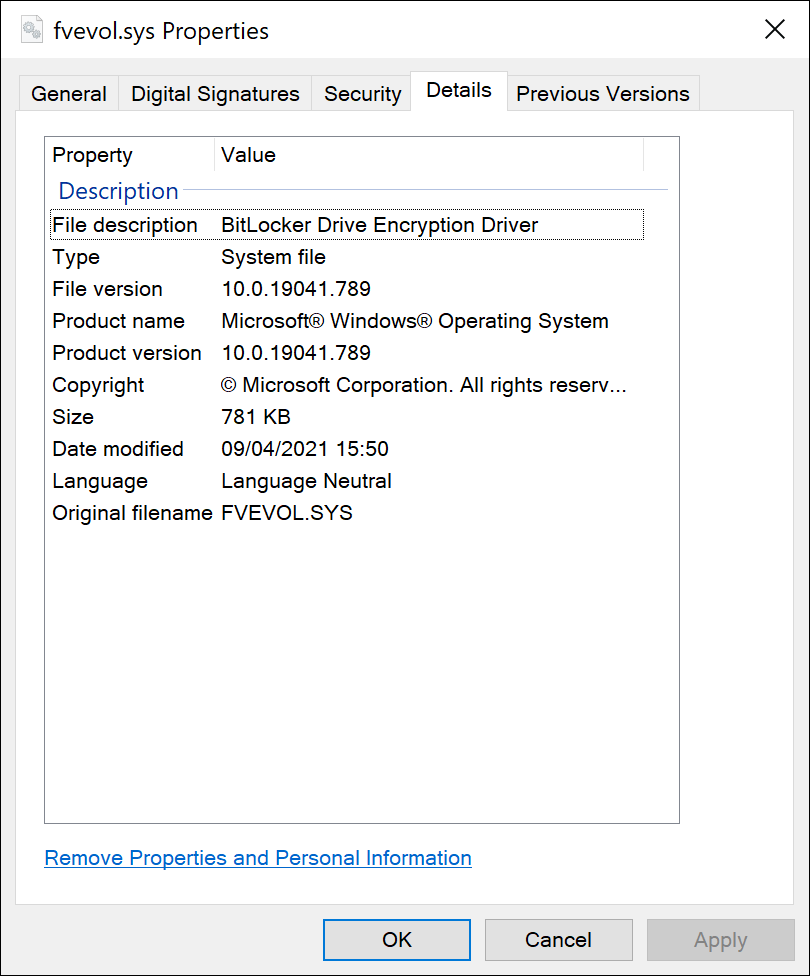
\includegraphics[scale=0.7]{../img/otherapproaches.bitlocker.fvevol.png}
	\caption[
		Properties of \texttt{fvevol.sys}
	]{
		Properties of \texttt{fvevol.sys} (screenshot from Windows Explorer). This file is usually located at \texttt{C:\textbackslash Windows\textbackslash System32\textbackslash drivers\textbackslash fvevol.sys}.
	}
	\label{fig:otherapproaches.bitlocker.fvevol}
\end{figure}

\autoref{fig:otherapproaches.bitlocker.driverentry} shows that the BitLocker driver filters only IRPs with certain major functions, skipping all other requests.

\begin{figure}[htb!]
	\center
	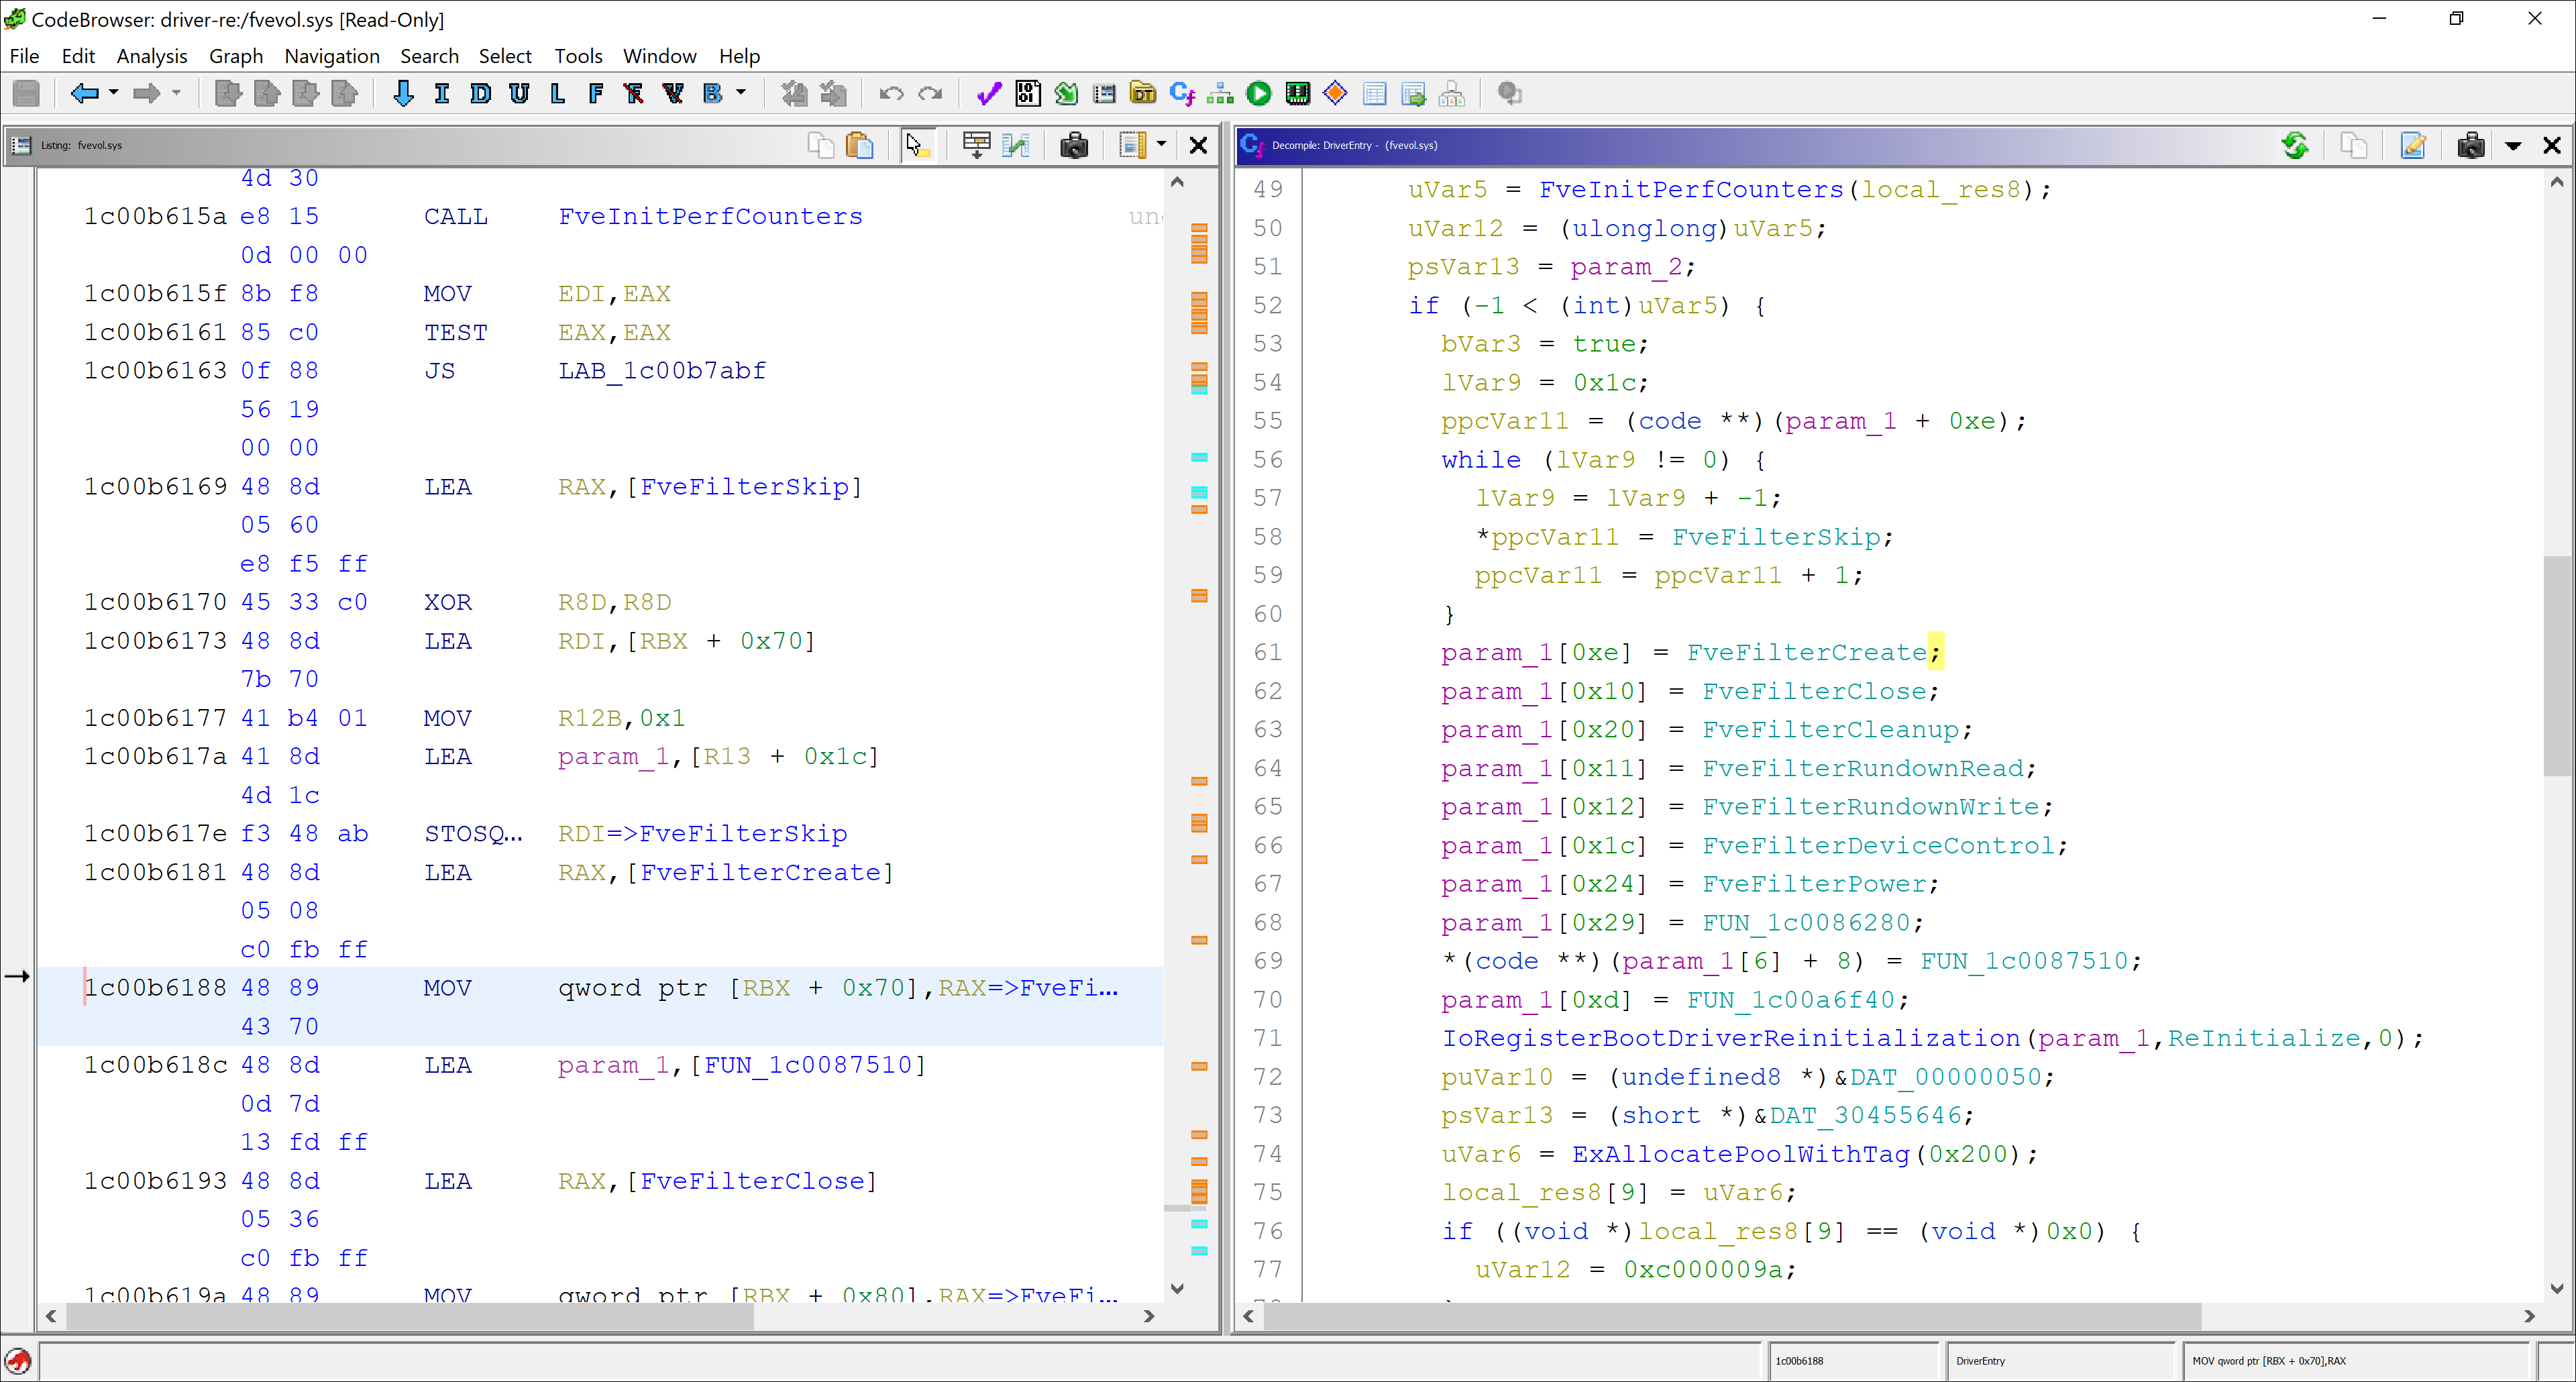
\includegraphics[scale=0.39]{../img/otherapproaches.bitlocker.driverentry.png}
	\caption[
		Assembly and disassembly of parts of the \texttt{DriverEntry} function
	]{
		Assembly and disassembly of parts of the \texttt{DriverEntry} function (screenshot from \href{https://www.ghidra-sre.org}{Ghidra}). Shown here is the definition of which function of the driver will be called when an IRP passes through it. These are called dispatch routines. The driver has to specify the different dispatch routine for each IRP major function. See \autoref{chap:ourapproach.final.genericdispatch} for more details on this initialization process.\\
		\texttt{fvevol.sys} only defines specific dispatch routines for the Create, Close, Cleanup, Read, Write, DeviceControl, Power, and PnP major functions. All others use a generic routine, which usually just forwards the IRP to the next driver in the stack (except for some error cases, where it fails the request).
	}
	\label{fig:otherapproaches.bitlocker.driverentry}
\end{figure}

From \autoref{fig:otherapproaches.bitlocker.xtsdecrypt} (and looking at more disassembled code, which is omitted here) it is clear that the BitLocker driver does not implement cryptographic functionality itself. Instead, it relies on the interface of another kernel driver.\footnote{\label{fn:otherapproaches.bitlocker.ksecdd} The documentation for the Windows Vista version of this interface can be found at \url{https://csrc.nist.gov/csrc/media/projects/cryptographic-module-validation-program/documents/security-policies/140sp891.pdf}.}

\begin{figure}[htb!]
	\center
	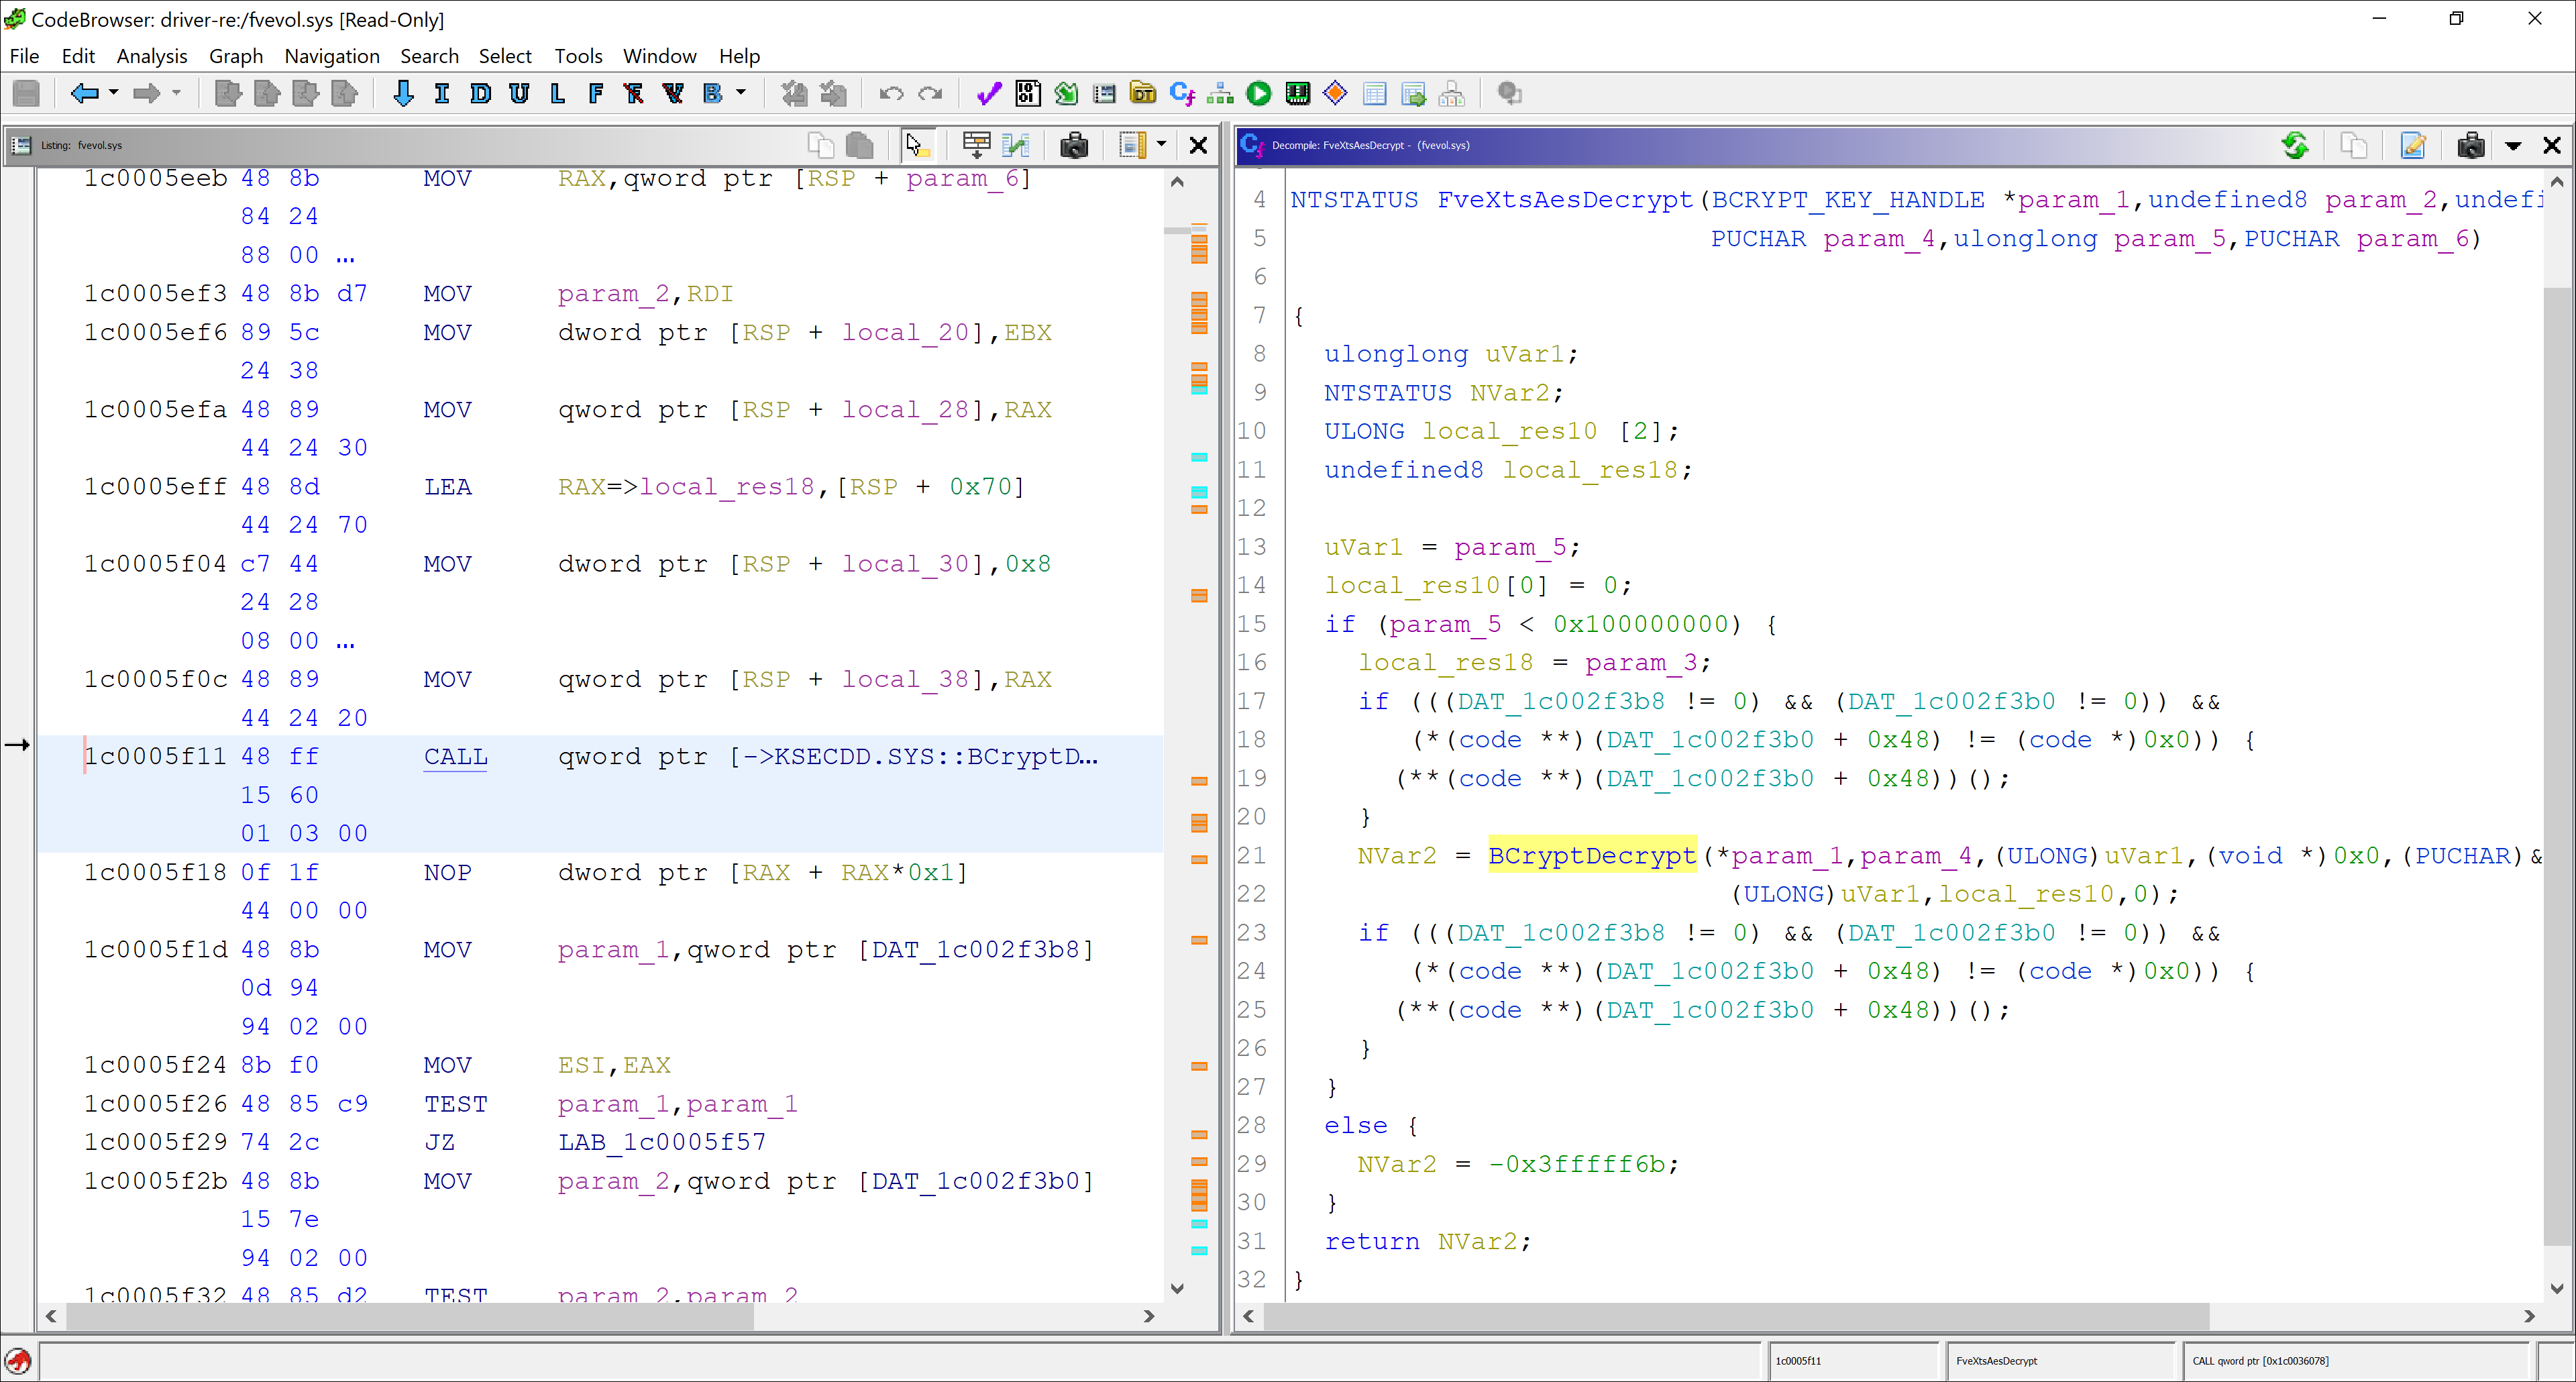
\includegraphics[scale=0.39]{../img/otherapproaches.bitlocker.xtsdecrypt.png}
	\caption[
		Assembly and disassembly of the \texttt{FveAesXtsDecrypt} function
	]{
		Assembly and disassembly of the \texttt{FveAesXtsDecrypt} function (screenshot from \href{https://www.ghidra-sre.org}{Ghidra}). \texttt{fvevol.sys} uses functions from \texttt{ksecdd.sys}, which is the ``Kernel Mode Security Support Provider Interface'', for all cryptographic functionality. Shown here is the implementation of AES-XTS decryption, which also makes use of this interface.
	}
	\label{fig:otherapproaches.bitlocker.xtsdecrypt}
\end{figure}

According to \cite{Kornblum2009}, ``Reverse engineering parts of the BitLocker system indicate that the system zeros out sensitive data as soon as they are no longer needed, consistent with good security practices.'' This is consistent with our findings presented in \autoref{fig:otherapproaches.bitlocker.deletekey}.

\begin{figure}[htb!]
	\center
	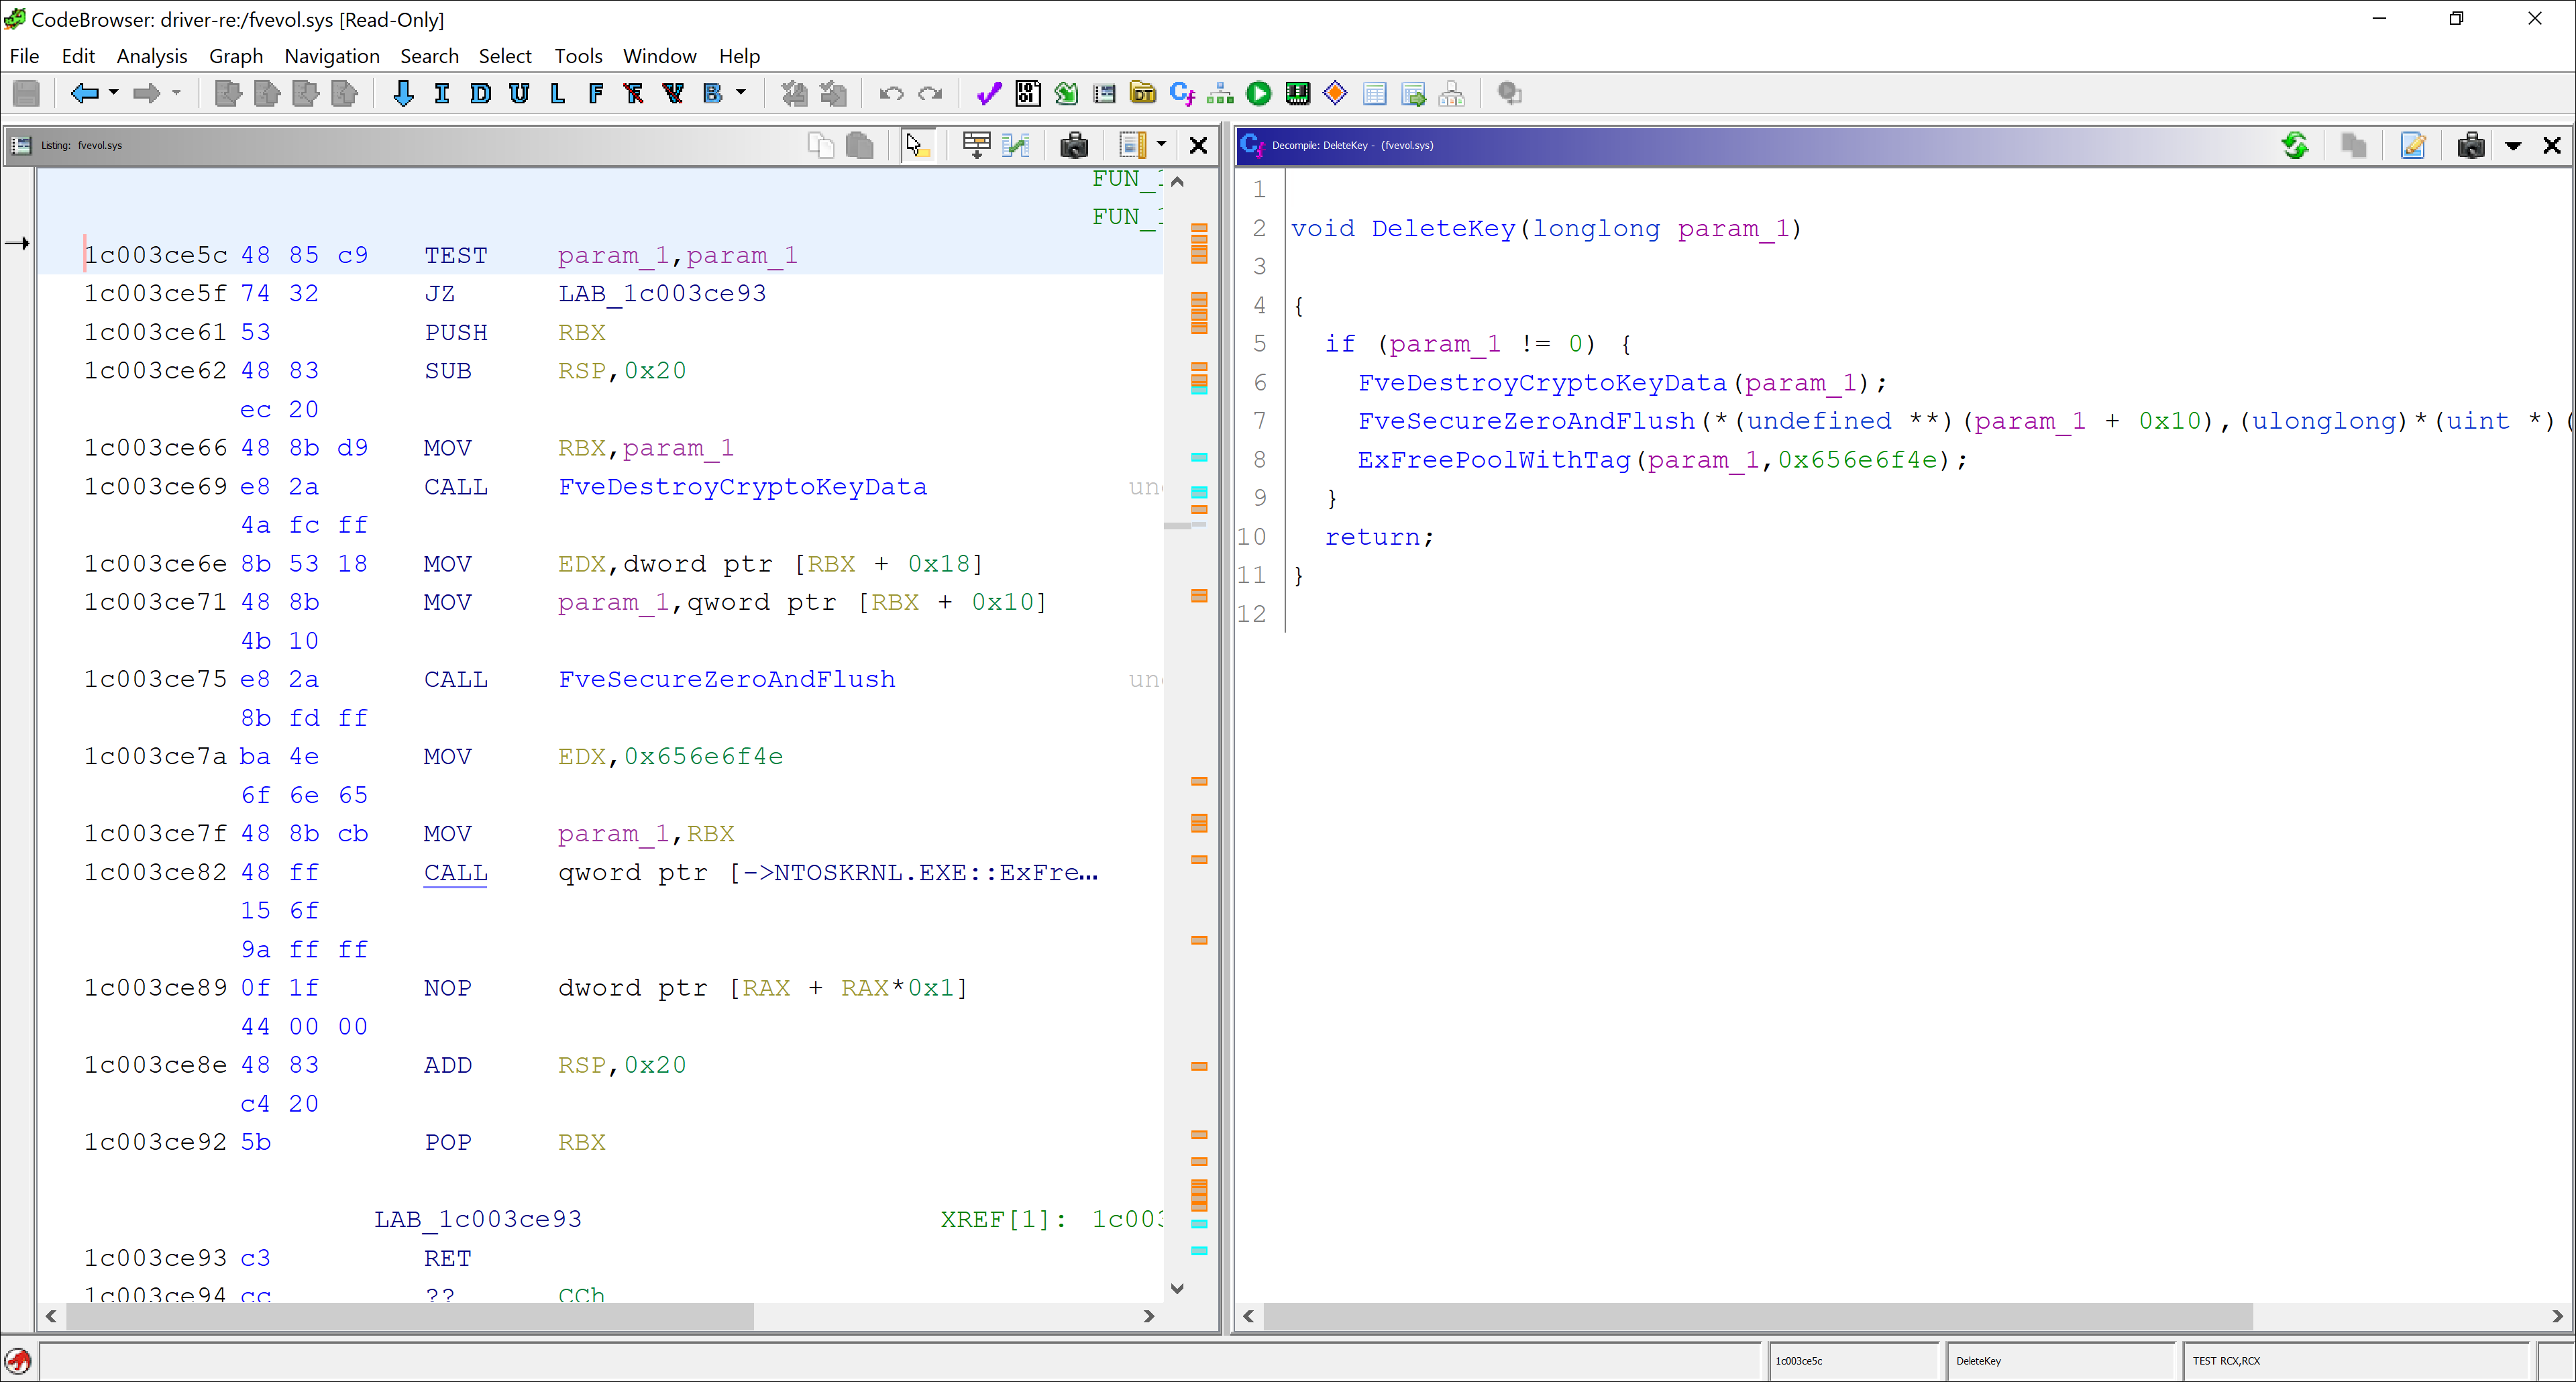
\includegraphics[scale=0.39]{../img/otherapproaches.bitlocker.deletekey.png}
	\caption[
		Assembly and disassembly of the \texttt{DeleteKey} function
	]{
		Assembly and disassembly of the \texttt{DeleteKey} function (screenshot from \href{https://www.ghidra-sre.org}{Ghidra}). The \texttt{FveDestroyCryptoKeyData} function notifies the \texttt{ksecdd.sys} driver that the key is no longer needed. \texttt{FveSecureZeroAndFlush} zeros out the key data and also calls \texttt{KeSweepLocalCaches}, which is not documented (but probably flushes the key data from the CPU's caches). \texttt{ExFreePoolWithTag} is basically a regular C \texttt{free} but for the Windows kernel.
	}
	\label{fig:otherapproaches.bitlocker.deletekey}
\end{figure}